\section{PROJECT IMPLEMENTATION}
\subsection{CAD Model Design} \label{sec:CAD Model Design}
When starting the project, we had a model of a quadruped from another project. This quadruped had 4 DoF (degrees of freedom) per leg like we wanted, but it had one major problem: the model complexity made modeling it very difficult. Therefore, our team decided to design a simple model in Dassault Solidworks, then import it into MATLAB Simulink. The latest model can be seen in Figure 1.
We then ported the model into MATLAB using exporting software offered by  Dassault Solidworks and we used the Simscape Multibody Simulink library in MATLAB to base the simulation of the robot.
Figure \ref{fig:cadmodel} shows the cad model. The legs are equivalent, but are given this specific pose to project our vision of how we see the cat stand in the future.
\begin{figure}[thpb]
    \parbox{\linewidth}{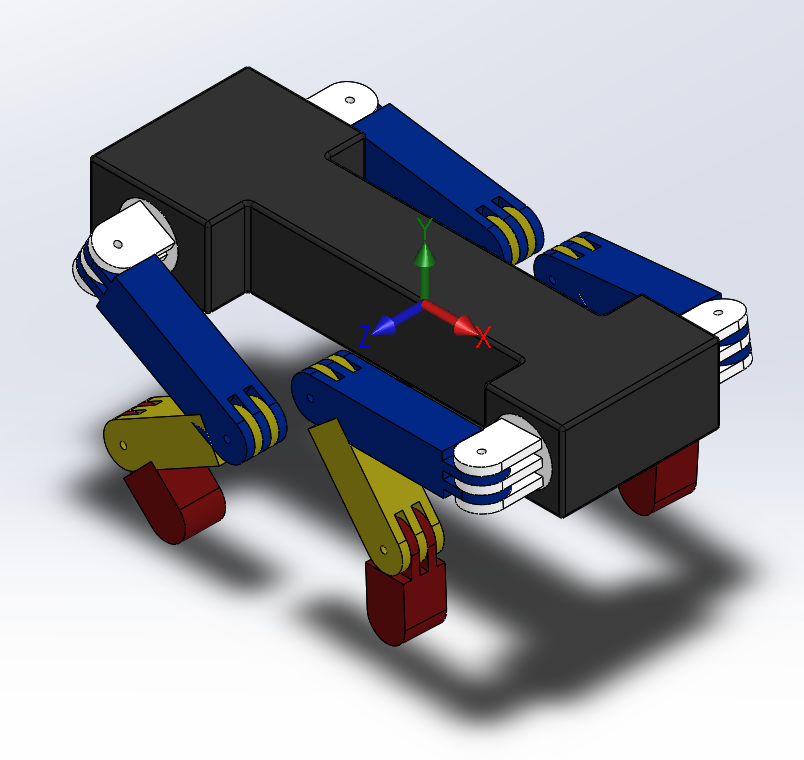
\includegraphics[width=\linewidth]{Figures/robot.png}}
    \caption{The CAD model of the simplified robot.}
    \label{fig:cadmodel}
\end{figure}

\subsection{Collision in Simulink 3D Model}
We used the Contact Forces Library to implement collision between parts of the robot and a plane we had placed underneath the robot. we used primitives called Sphere-to-plane collision blocks, which allow us to model a sphere to plane collision in SimuLink. However, without any control inputs on the legs we can't keep the legs straight to demonstrate a standing behavior of the quadruped. We did achieve a dangling pose and a crashing one for the robot, though.

Aiming to fully constraining the model (adding self-collision and body-plane collision) would send us off on a path that may derail us from reaching our reach goal. Figure \ref{fig:collision} shows an older model colliding with the floor.
\begin{figure}[thpb]
    \parbox{\linewidth}{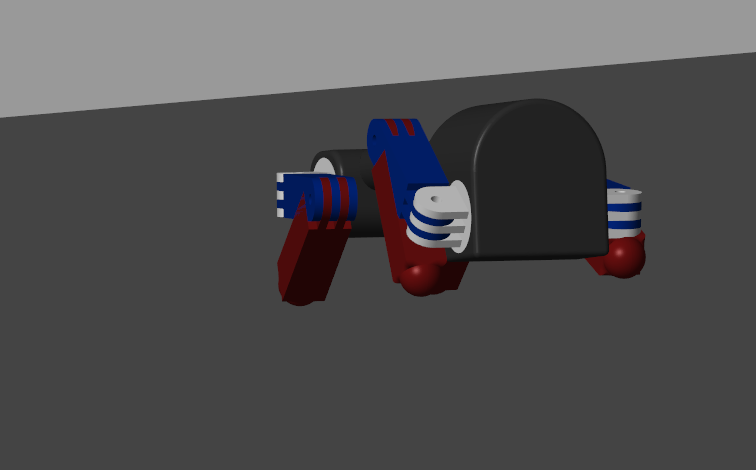
\includegraphics[width=\linewidth]{Figures/ContactModel.png}}
    \caption{The cat crashing into the floor after falling from a height.}
    \label{fig:collision}
\end{figure}

\subsection{DH-Parameters and Validation} \label{sec:dhparams}
\begin{figure}[thpb]
    \parbox{\linewidth}{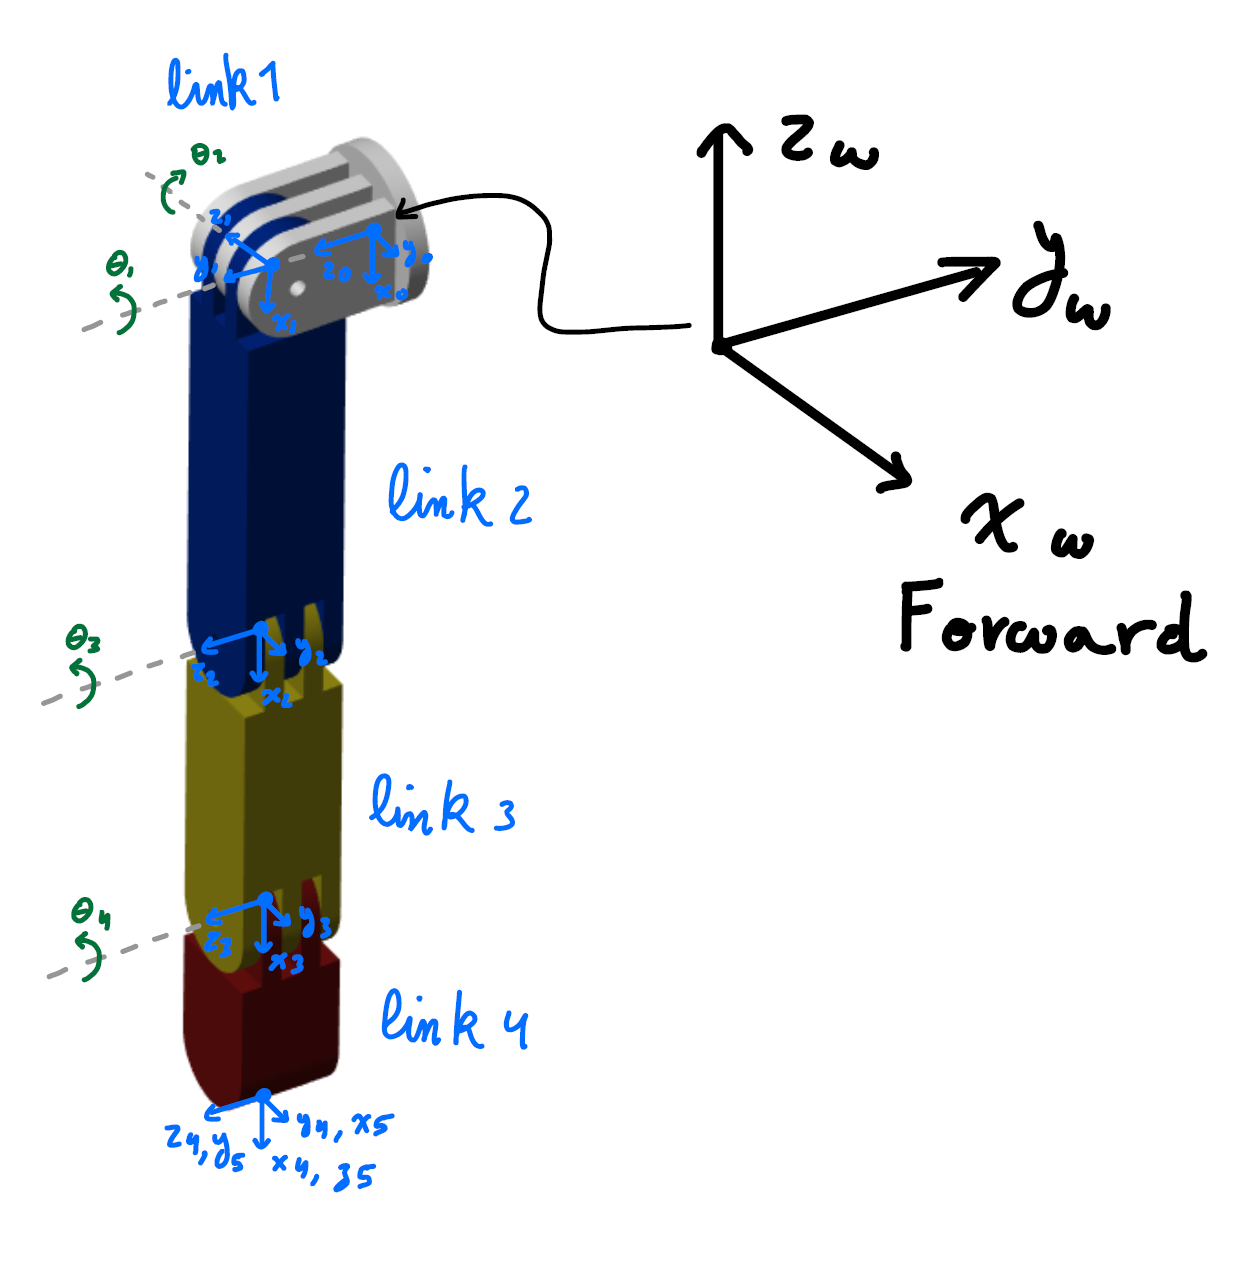
\includegraphics[width=\linewidth]{Figures/dhframes.png}}
    \caption{The chosen DH frames.}
    \label{fig:dhframes}
\end{figure}

The most important set of calculations is the DH-parameters. This computation is the precursor of all the work that follows in terms of forward kinematics and dynamic modeling. Since, in our model, all legs are designed to be similar, we only need to specify the DH-parameters for one leg. Figure \ref{fig:dhframes} shows the chosen frames. The rationale behind choosing the robot's frame $F_w$ as having the z-axis pointing upward as opposed to having it point in the direction of the axis of the first joint is to make subsequent computations of the dynamic model intuitive, especially when gravity is to be considered. This design choice gives us some sort of intuitive assumption that gravity points down by default (which will also be made to change with the orientation of the robot).
Table \ref{tab:dhparams} shows the DH-table that situates the frames with respect to the robot's world frame as shown in figure \ref{fig:dhframes}. The first two rows correspond to the transformation from the world frame to the first joint's frame, the next four are those that propagate the frame orientations based on the values of the joint angles, and the last one orients the approach vector along the final link's axis, which is customary to do, in the literature, and useful, in practice.

\begin{table}
\caption{DH-Parameters}
\label{tab:dhparams}
\begin{center}
\begin{tabular}{ | c | c | c | c | c |} 
\hline
link & $\theta_i$ & $d_i$ & $a_i$ & $\alpha_i$ \\
\hline
Rot1 & 0 & 0 & 0 & $\frac{\pi}{2}$ \\
\hline
Rot2 & $-\frac{\pi}{2}$ & 0 & 0 & 0 \\
\hline
1    & $\theta_1$ & 30  & 0  & $\frac{\pi}{2}$  \\
\hline
2    & $\theta_2$  & 0  & 100 & $-\frac{\pi}{2}$  \\
\hline
3    & $\theta_3$  & 0  & 75  & 0 \\
\hline
4    & $\theta_4$  & 0  & 50  & 0 \\
\hline
5    & $\frac{\pi}{2}$  & 0  & 0  &  $\frac{\pi}{2}$ \\
\hline
\end{tabular}
\end{center}
\end{table}

Figure \ref{fig:dhvalidation} shows how we validated those DH-parameters.

\begin{figure}[thpb]
    \parbox{\linewidth}{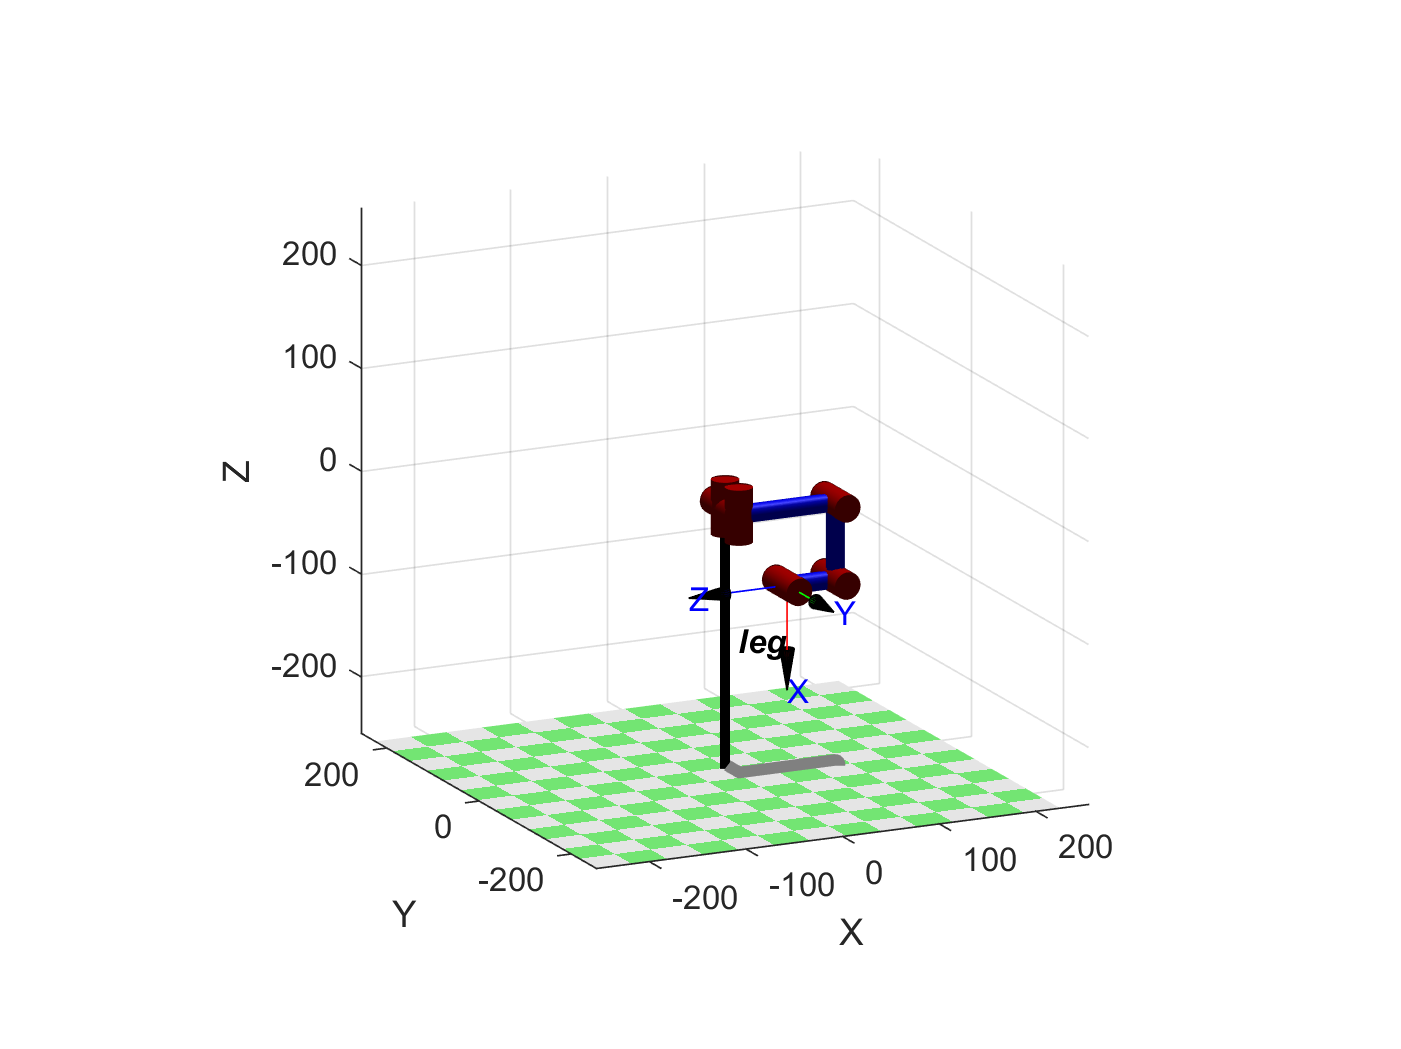
\includegraphics[width=\linewidth]{Figures/dhvalidation.png}}
    \caption{The plot that validates our DH-parameters. The configuration $\theta$ was set to [$\frac{\pi}{2}$ 0 -$\frac{\pi}{2}$ -$\frac{\pi}{2}$] to give the expected configuration in a plot. The Robotics Toolbox for MATLAB was used to generate this plot.}
    \label{fig:dhvalidation}
\end{figure}

\subsection{Forward Kinematics}
Given those DH-parameters shown in \ref{sec:dhparams}, it is almost trivial to compute the forward kinematics. A MATLAB function is setup for reuse across this project. The MATLAB function returns all the intermediate frames in a 3D matrix, for convenience and efficiency. This function will be used once in the Jacobian computation and the 3D matrix is used more than once, which removes the overhead due to calling this function and computing the forward kinematics.

\subsection{Inverse Kinematics}
At first we had decided to calculate the inverse kinematics using a geometric approach, and we actually did manage to do so. However, after doing some research, we decided to use a different approach. By calculating the inverse velocity kinematics, we can represent a trajectory in task-space, and interpolate the intermediate joint angles from there, as explained in \cite{spong2006robot}, and in Section \ref{sec:trajectories} Trajectories and Controller.


\subsection{The Jacobian}
The Jacobian of an individual leg is the single most important aspect in the process of dynamically modeling the quadruped in question. In fact, we need to be able to compute more than one Jacobian for each configuration, one for each link in the manipulator/leg.
For this purpose, we referred to the book "Robot Modeling and Control" \cite{spong2006robot}, which gives a cookbook method of computing the Jacobian for a point along one of the links of an n-link manipulator. Based on that, we created a function that takes the index of the joint and returns a corresponding 6x4 Jacobian matrix. For the purpose of dynamically modeling the robot, we do not need the matrix to be square. However, for the purpose of task-space trajectory tracking we need the pseudo-inverse.

\subsection{The Dynamics}
In order to control the robot using torque, we need to provide a signal that takes into account the dynamics of the system, hence the need for a dynamical model. To acquire one, we followed the cookbook method shown in the "Robot Modeling and Control" \cite{spong2006robot} and \cite{murray2017mathematical}. We used the first resource to get the general equations and the second to resolve some ambiguity about whether the \textbf{Inertia Tensors} used in the equations were defined with respect to the center of the link or its hinge point. Both resources are complementary and discuss examples that highlight different nuances.
From \cite{spong2006robot}, we got the general equation of the Inertia Matrix:
$$
M(q) = \sum_{i=1}^n \{m_i J_{vi}(q)^T J_{vi}(q) + J_{\omega i}(q)^T R_i(q) I_i R_i(q)^T J_{\omega i}(q)\},
$$
where i is in the index of the center of mass of the $i^{th}$ link, $J_{vi}$ the linear velocity part of the Jacobian, and  $J_{\omega i}$ the rotational part of it for the center of mass of the $i^{th}$ link. In the rotational part of the equation, $I_i$ is the constant inertia tensor defined with respect to the $i^{th}$ link, and $R_i$ the rotation matrix that aligns the inertia tensor to the link with respect to the base-frame. $R_i(q) I_i R_i(q)^T$ is thus the inertia tensor of the $i^{th}$ link with respect to the base frame, which is a function of q.
We acquired the inertia tensors from the SolidWorks model of the leg that we had designed and the rotation was computed by combining the rotation that transforms coordinates from the base to the end of the $i^{th}$ link and another which we designed by hand so that the inertia tensor is aligned with the one represented in SolidWorks. The process was iterative, but we could not validate whether we had the correct configuration until we were able to test it on the model itself.
The other terms are easy to acquire from the properties of the robot, as well as the Jacobian computations.
Then, the elements of the Coriolis and Centrifugal forces matrix were computed by using M's elements and the following equation:
$$
c_{kj} = \sum_{i=1}^n \{\frac{\partial d_{kj}}{\partial q_i} + \frac{\partial d_{ki}}{\partial q_j} - \frac{\partial d_{ij}}{\partial q_k} \}\dot{q_i},
$$
where $c_{kj}$ is the intersection of M's $k^{th}$ row and M's $j^{th}$ column.
Then, to get the symbolic G vector, we get the system's potential energy as follows:
$$
P = \sum_{i=1}^n m_i g^T r_{c_i}
$$
where $g^T r_{c_i}$ is the project of the distance to the base-frame of the $i^{th}$ link. We leave the variable g parametric, that is, we let be a symbolic vector and based on the situation in which the arm/leg find itself in, we would then set this g accordingly to counter the effect of gravity on the arm.
Differentiating this equation with respect to the vector of joint values, we obtain the G vector, which is the gravity vector of a manipulator. The following shows the equation we referred to:
$$
g_k = \frac{\partial P}{\partial q_k}
$$

The resulting matrices can be used to express the dynamic model of the robot which goes like this:
$$
M(q) \ddot{q} + C(q, \dot{q}) \dot{q} + G = \tau
$$

Implementation wise, the M, C and G matrices were computed in a file called generatingDynamics.m, which initializes the parameters like weights and inertia tensors and then calls another function which returns the Jacobians for the chosen center of mass, in addition to the rotation that aligns the corresponding inertia matrix and $r_{c_i}$ vectors (the vector that indicates the location of the center of mass of the $i^{th}$ link with respect to the base). Once the matrices are computed, they are turned from symbolic matrices, which are very slow to evaluate, into matlab functions using the matlabFunction routine which is part of the symbolic toolbox. The result is a set of functions, computeM, computeC and computeG which combined run at an average of 25 milliseconds, which is good enough for simulation. Figure \ref{fig:dhframes} also shows the frame in which the dynamic model is shown. Note that in this frame, the gravity can sometimes be in another orientation than the negative $z_world$ vector.

% \section{Hypothesis}
% As we were thinking of the different ingredients to our rather simple method of making the robot walk, a hypothesis was brewing in our minds. \\
% \textbf{Hypothesis:} The robot, augmented with the above modeling and compensation, will be able to stand, and perform a few steps on a smooth plane before stumbling.

